\section{Systems Optimization for SSMs}
\label{sec:systems}

We describe several systems optimizations for SSMs, in particular the Mamba-2 architecture, for large-scale efficient training and inference.
In particular, we focus on tensor parallel and sequence parallel for large-scale training, as a well variable-length sequences for efficient finetuning and inference.

\subsection{Tensor Parallel}
\label{subsec:tp}

Tensor parallelism (TP)~\citep{shoeybi2019megatron} is a model parallelism technique that splits each layer (e.g., attention, MLP) to run on multiple accelerators such as GPUs.
This technique is widely used to train most large models~\citep{brown2020language, chowdhery2022palm, touvron2023llama, touvron2023llama2}  on GPU clusters where each node typically has 4-8 GPUs with fast networking such as NVLink.
TP was originally developed for the Transformer architecture, and it is not straight-forward to adapt it other architecture.
We first show the challenge of using TP with the Mamba architecture, and the show how the Mamba-2 architecture is designed to make TP efficient.

Recall the Mamba architecture, with a single input $u \in \mathbb{R}^{L \times d}$ (no batching for simplicity), input projection matrices $W^{(x)}, W^{(z)} \in \mathbb{R}^{d \times ed}$ where $e$ is the expansion factor (typically 2), and output projection matrix $W^{(o)} \in \mathbb{R}^{ed \times d}$:
\begin{align*}
   x &= u {W^{(x)}}^\top \in \mathbb{R}^{L \times ed} \\
   z &= u {W^{(z)}}^\top \in \mathbb{R}^{L \times ed} \\
   x_c &= \mathrm{conv1d}(x) \in \mathbb{R}^{L \times ed} \quad \text{(depthwise, independent along $d$)} \\
   \Delta, B, C &= \text{low-rank projection}(x_c) \\
   y &= SSM_{A, B, C, \Delta}(x_c) \in \mathbb{R}^{L \times ed} \quad \text{(independent along $d$)} \\
   y_g &= y \cdot \phi(z)  \quad \text{(gating, e.g., with $\phi$ being SiLU)} \\
  \mathrm{out} &= y_g {W^{(o)}}^\top \in \mathbb{R}^{L \times d}.
\end{align*}
With TP, suppose that we want to split the computation along 2 GPUs. It is easy to split the input projection matrices $W^{(x)}$ and $W^{(z)}$ into two partitions each of size $d \times \frac{ed}{2}$.
Then each GPU would hold half of $x_c$ of size $L \times \frac{ed}{2}$.
However, we see that since $\Delta, B, C$ are functions are $x_c$, so we would need an extra all-reduce between the GPUs to get the whole of $x_c$ before computing $\Delta, B, C$.
After that the two GPUs can compute the SSM in parallel since they are independent along $d$.
At the end, we can split the output projection matrices $W^{(o)}$ into two partitions each of size $\frac{ed}{2} \times d$, and do an all-reduce at the end.
Compared to Transformers, we would incur two all-reduces instead of one, doubling the time spent in communication. For large-scale Transformers training, communication might already take a significant fraction of time (e.g. 10-20\%), and doubling communication would make Mamba not as efficient for large-scale training.

With Mamba-2, our goal is to have only one all-reduce per block, similar to attention or MLP blocks in Transformers.
As a result, we have the projection to get $\Delta, B, C$ directly from $u$ instead of from $x_c$, allowing us to split these projection matrices.
This implies that we have different sets of $\Delta, B, C$ on different GPUs, which is equivalent to having several ``groups'' of $\Delta, B, C$ on a larger ``logical GPU''.
Moreover, we use GroupNorm within each block, with number of groups divisible by the TP degree, so that the GPUs in a TP group do not have a communicate within the block:
\begin{align*}
   x &= u {W^{(x)}}^\top \in \mathbb{R}^{L \times ed} \\
   z &= u {W^{(z)}}^\top \in \mathbb{R}^{L \times ed} \\
   \Delta, B, C &= \text{projection}(u) \quad \text{(one or more groups of $\Delta, B, C$ per GPU)} \\
   x_c &= \mathrm{conv1d}(x) \in \mathbb{R}^{L \times ed} \quad \text{(depthwise, independent along $d$)} \\
   y &= SSM_{A, B, C, \Delta}(x_c) \in \mathbb{R}^{L \times ed} \quad \text{(independent along $d$)} \\
   y_g &= y \cdot \phi(z)  \quad \text{(gating, e.g., with $\phi$ being SiLU)} \\
   y_n &= \mathrm{groupnorm}(y_g) \quad \text{(number of groups divisible by degree of tensor parallel)} \\
   \mathrm{out} &= y_g {W^{(o)}}^\top \in \mathbb{R}^{L \times d}.
\end{align*}

We see that we only need to split the input projection matrices, and the output projection matrices, and only need to do all-reduce at the end of the block. This is similar to the design of TP for attention and MLP layers.
In particular, if we have TP degree 2, we would split $W^{(x)} = [W^{(x)}_1, W^{(x)}_2]$ with $W^{(x)}_i \in \mathbb{R}^{d \times ed/2}$,
$W^{(z)} = [W^{(z)}_1, W^{(z)}_2]$ with $W^{(z)}_i \in \mathbb{R}^{d \times ed/2}$,
and $W^{(o)} = \begin{bmatrix} W^{(o)}_1 \\ W^{(o)}_2 \end{bmatrix}$ with $W^{(o)}_i \in \mathbb{R}^{ed/2 \times d}$.
For $i = 1, 2$, the TP Mamba-2 layer can be written as:
\begin{align*}
   x^{(i)} &= u {W^{(x)}_i}^\top \in \mathbb{R}^{L \times ed / 2} \\
   z^{(i)} &= u {W^{(z)}_i}^\top \in \mathbb{R}^{L \times ed / 2} \\
   \Delta^{(i)}, B^{(i)}, C^{(i)} &= \text{projection}(u) \quad \text{(one or more groups of $\Delta, B, C$ per GPU)} \\
   x_c^{(i)} &= \mathrm{conv1d}(x^{(i)}) \in \mathbb{R}^{L \times ed / 2} \\
   y^{(i)} &= SSM_{A, B, C, \Delta}(x_c^{(i)}) \in \mathbb{R}^{L \times ed/2}  \\
   y_g^{(i)} &= y^{(i)} \cdot \phi(z^{(i)})  \\
   y_n^{(i)} &= \mathrm{groupnorm}(y_g^{(i)}) \quad \text{(number of groups divisible by degree of tensor parallel)} \\
   \mathrm{out}^{(i)} &= y_g^{(i)} {W^{(o)}_i}^\top \in \mathbb{R}^{L \times d / 2} \\
   \mathrm{out} &= \sum_i \mathrm{out}^{(i)}. \quad \text{(summing outputs from all GPUs with an all-reduce)}
\end{align*}
We illustrate tensor parallel with Mamba-2 in~\cref{fig:mamba2_parallelism} (\emph{Left}).
\begin{figure}[!t]
\centering
\begin{minipage}{.4\linewidth}%
  \centering
  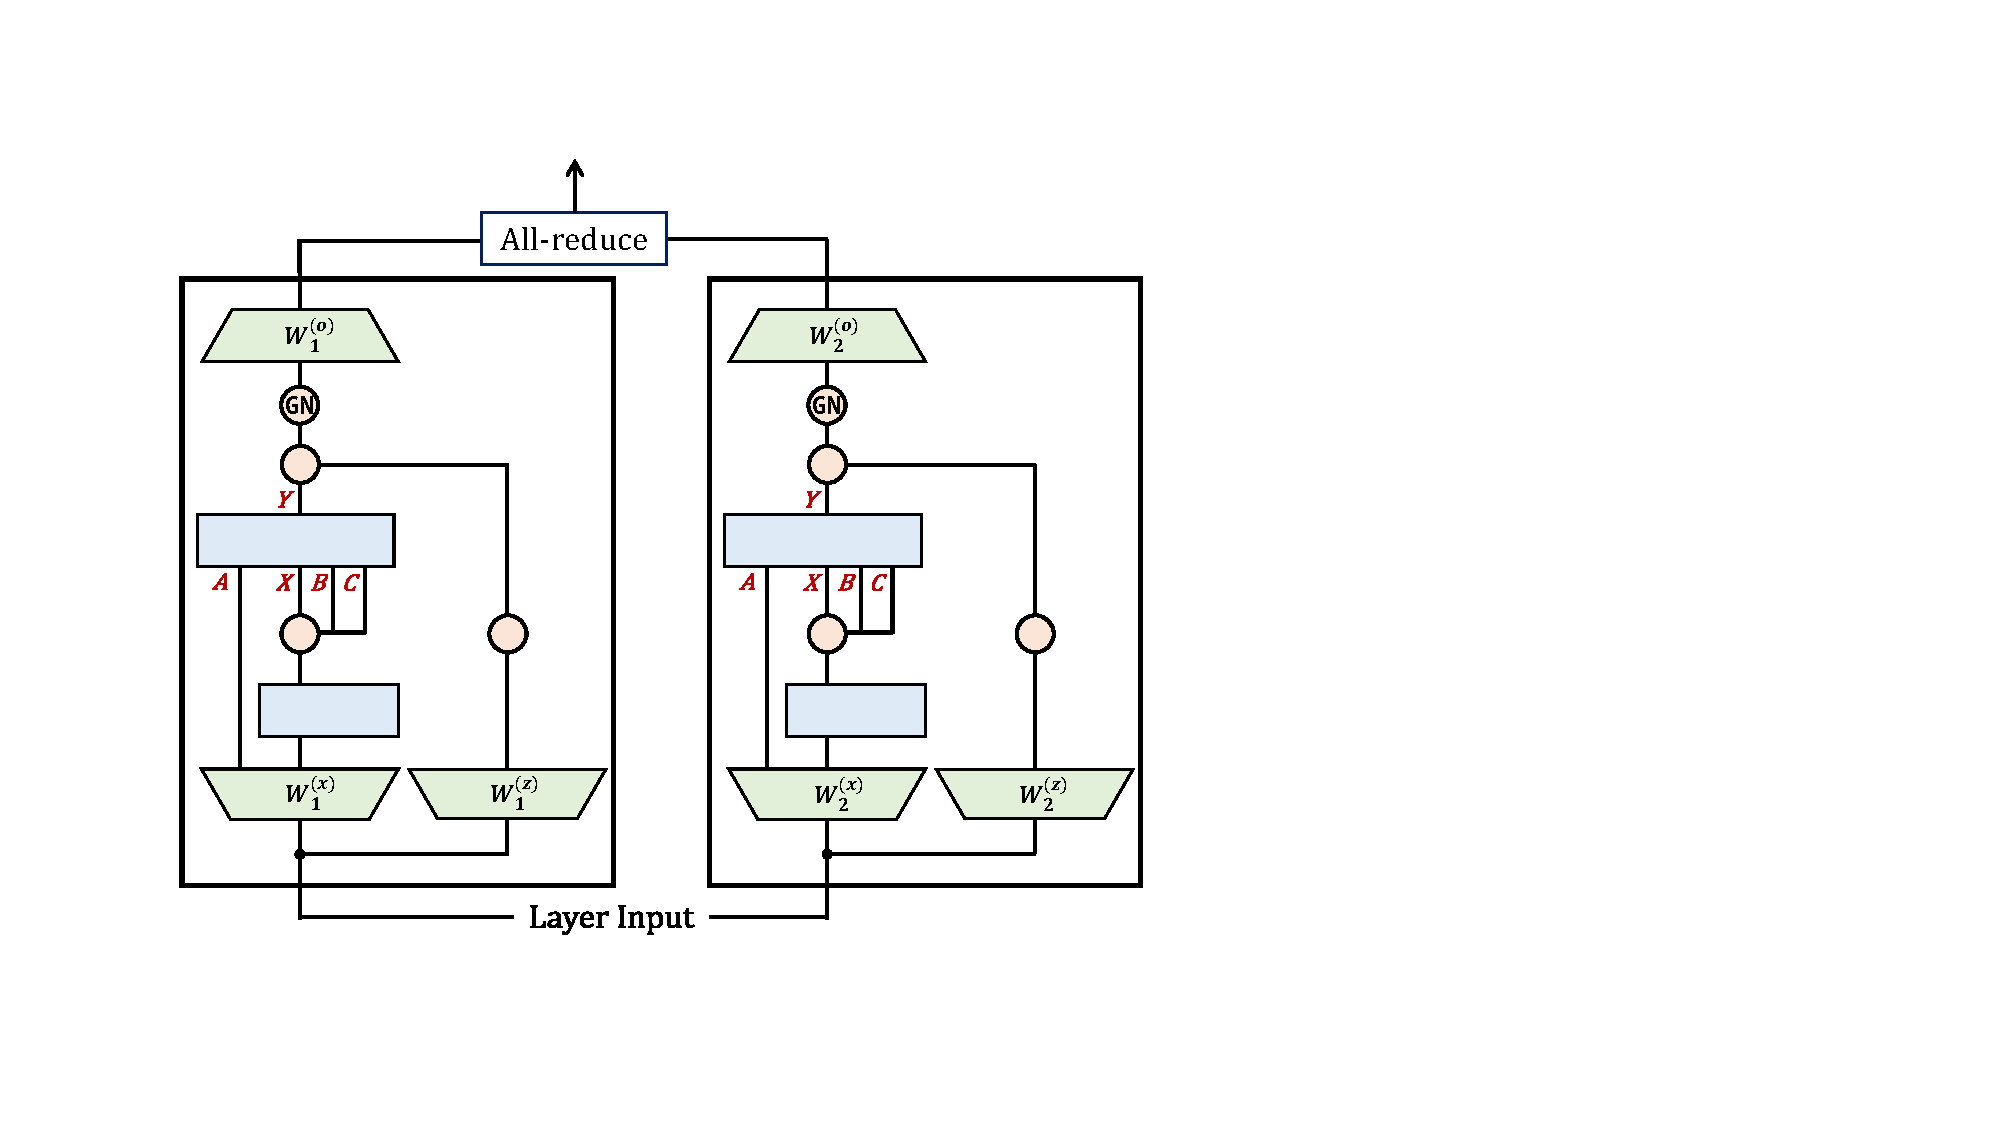
\includegraphics[width=\linewidth]{fig/mamba_tp.pdf}
\end{minipage}
\hfill
\begin{minipage}{.59\linewidth}%
  \centering
  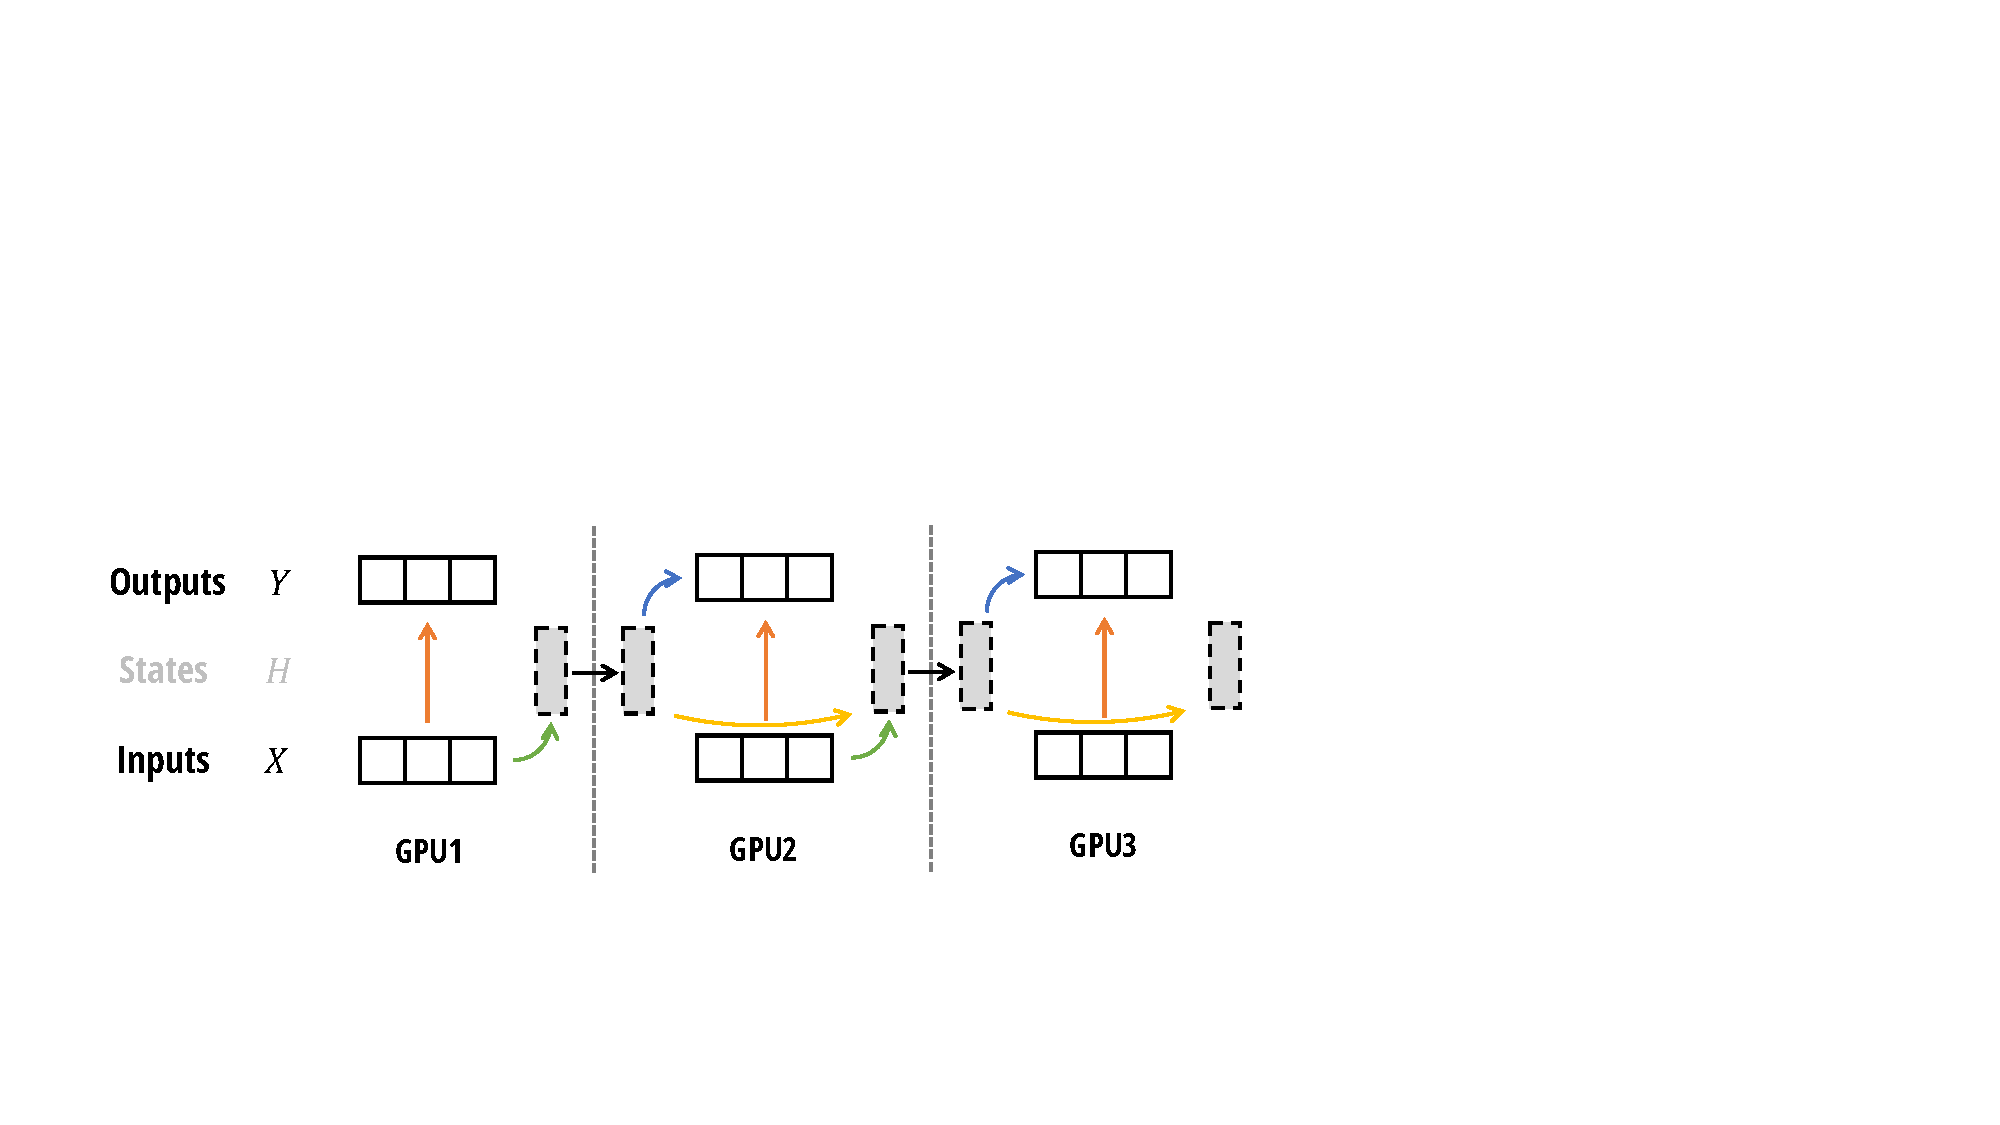
\includegraphics[width=\linewidth]{fig/mamba_cp.pdf}
\end{minipage}
\caption{
  (\textbf{Parallelism with the Mamba-2 Block}.)
  (\emph{Left}: \textbf{Tensor Parallelism})
  We split the input projection matrices $W^{(x)}, W^{(z)}$ and the output projection matrix $W^{(o)}$.
  Each SSM head $(A, B, C, X) \mapsto Y$ lives on a single device.
  Choosing GroupNorm for the final normalization layer avoids extra communication.
  We need one all-reduce per layer, just like the MLP or attention blocks in a Transformer.
  (\emph{Right}: \textbf{Sequence/Context Parallelism})
  Analogous to the SSD algorithm, with multiple devices, we can split along the sequence dimension. Each device computes the state of its sequence, then pass that state to the next GPU.
}
\label{fig:mamba2_parallelism}
\end{figure}

\subsection{Sequence Parallelism}
\label{subsec:sp}

For very long sequences, we might need to split the input and activation to different GPUs along the sequence length dimension.
There are two main techniques:
\begin{enumerate}
\item Sequence parallelism (SP) for the residual and normalization operations: first proposed by~\citet{korthikanti2023reducing}, this technique decomposes the all-reduce in TP as reduce-scatter and all-gather. Noticing that the residual and normalization operations are repeated on the same input for all GPUs in the same TP group, SP splits the activations along the sequence length dimension by performing: reduce-scatter, residual and normalization, then all-gather.

Since the Mamba-2 architecture uses the same residual and normalization structure, SP applies without modification.

\item Sequence parallelism for the token-mixing operations (attention or SSM), also known as ``context parallelism'' (CP).
Several techniques have been developed for attention layer (e.g., Ring attention~\citep{liu2023ring, liu2024world}), with sophisticated load-balancing technique~\citep{brandon2023striped}.
The difficulty with sequence parallelism in attention is that we can split queries and keys into block, but each query block needs to interact with key blocks, leading to communication bandwidth quadratic in the number of workers.

With SSMs, we can split the sequence in a simple manner: each worker takes an initial state, compute the SSM with respect to their inputs, return the final state, and pass that final state to the next worker.
The communication bandwidth is linear in the number of workers.
This decomposition is exactly the same as the block-decomposition in the SSD algorithm (\cref{fig:ssd-algorithm}) to split into blocks / chunks.
We illustrate this context parallelism in~\cref{fig:mamba2_parallelism} (\emph{Right}).

\end{enumerate}

\subsection{Variable Length}
\label{subsec:varlen}

While pretraining often uses the same sequence lengths for the batch, during finetuning or inference, the model might need to process different input sequences of different lengths.
One naive way to handle this case is to right-pad all sequences in the batch to the maximum length, but this can be inefficient if sequences are wildly different lengths.
For transformers, sophisticated techniques have been develop to avoid padding and do load-balancing between GPUs~\citep{zeng2022boosting, zhai2023bytetransformer}, or packing multiple sequences in the same batch and adjust the attention mask~\citep{ding2024fewer, pouransari2024dataset}.
With SSMs and Mamba in particular, we can handle variable sequence lengths by simply treating the whole batch as one long sequence, and avoid passing the states between individual sequences.
This is equivalent to simply setting $A_t = 0$ for tokens $t$ at the end of one sequence to prevent it from passing information to the token $t + 1$, which belongs to a different sequence.
